%%%%%%%%%% !TEX program = pdflatex %%%%%%%%%%
% !TEX program = pdflatex
\documentclass[a4paper,12pt,openany,twoside]{book}

% 当目录多于1页时,使用\thispagestyle{empty}和\pagestyle{empty},都无法完全清除目录的页眉页脚格式,需要使用到下面的\AtBeginDocument{}代码
\AtBeginDocument{
	\addtocontents{toc}{\protect\thispagestyle{empty}}%
	\addtocontents{lof}{\protect\thispagestyle{empty}}%
}

                                           % 如果论文超过60页 可以使用twoside 双面打印
% !TEX program = pdflatex
% !Mode:: "TeX:UTF-8"
%  Authors: 杜家宜   Jiayi Du: Max_dujiayi@gmail.com     湖南大学2010级计算机科学与技术专业博士生

%%%%%%%%%% Package %%%%%%%%%%%%
\usepackage[chapter]{algorithm}
\usepackage{pdfpages}% 方便插入签字版权页
%\usepackage{algorithmic}

\usepackage{algpseudocode}

\usepackage{graphicx}                       % 支持插图处理
\usepackage{geometry}
\geometry{left=2.5cm,right=2.5cm,top=2cm,bottom=2.5cm,footskip=1.1cm,headsep=0.7cm,head=0.4cm}
% 支持版面尺寸设置
\usepackage{titlesec}                       % 控制标题的宏包
\usepackage{titletoc}                       % 控制目录的宏包
\usepackage{fancyhdr}                       % fancyhdr宏包 支持页眉和页脚的相关定义
\usepackage[UTF8]{ctex}                    % 支持中文显示
\usepackage{cite}
\usepackage{color}                          % 支持彩色
\usepackage{amsmath}                        % AMSLaTeX宏包 用来排出更加漂亮的公式
\usepackage{amssymb}                        % 数学符号生成命令
\usepackage{mathrsfs}                       % Add by Lijianmin
\usepackage{cases}
\usepackage[below]{placeins}                %允许上一个section的浮动图形出现在下一个section的开始部分,还提供\FloatBarrier命令,使所有未处理的浮动图形立即被处理
\usepackage{flafter}                        % 使得所有浮动体不能被放置在其浮动环境之前,以免浮动体在引述它的文本之前出现.
\usepackage{multirow}                       % 使用Multirow宏包,使得表格可以合并多个row格
\usepackage{booktabs}                       % 表格,横的粗线;\specialrule{1pt}{0pt}{0pt}
\usepackage{longtable}                      % 支持跨页的表格。
\usepackage{tabularx}                       % 自动设置表格的列宽
\usepackage{setspace}
\usepackage{subfigure}                      % 支持子图 %centerlast 设置最后一行是否居中
\usepackage[subfigure]{ccaption}            % 支持子图的中文标题

%\usepackage{hologo}
%\usepackage[super]{gbt7714}

\usepackage[sort&compress,numbers]{natbib}  % 支持引用缩写的宏包
\usepackage{enumitem}                       % 使用enumitem宏包,改变列表项的格式
\usepackage{calc}                           % 长度可以用+ - * / 进行计算
\usepackage{txfonts}                        % 字体宏包
\usepackage{bm}                             % 处理数学公式中的黑斜体的宏包
\usepackage[amsmath,thmmarks,hyperref]{ntheorem}  % 定理类环境宏包,其中 amsmath 选项用来兼容 AMS LaTeX 的宏包
\usepackage{CJKnumb}                        % 提供将阿拉伯数字转换成中文数字的命令
\usepackage{indentfirst}                    % 首行缩进宏包
\usepackage{CJKutf8}                        % 用在UTF8编码环境下,它可以自动调用CJK,同时针对UTF8编码作了设置。
\usepackage{CJK}
\usepackage{fancyhdr}
\usepackage{lastpage}
\usepackage{layout}
\usepackage[titles,subfigure]{tocloft}      %控制生成的表格和图片的目录格式
%\usepackage{caption}
% Add by Lijianmin
%\usepackage{hypbmsec}                      % 用来控制书签中标题显示内容
%\usepackage{bbding}
%如果您的pdf制作中文书签有乱码使用如下命令,就可以解决了
%Modified by Lijianmin
\usepackage[unicode,               % pdflatex, pdftex 这里决定运行文件的方式不同
%\usepackage[dvipdfm, unicode,               % pdflatex, pdftex 这里决定运行文件的方式不同
pdfstartview=FitH,
%CJKbookmarks=true,
bookmarksnumbered=true,
bookmarksopen=true,
colorlinks=true,
pdfborder={0 0 1},
citecolor=black,
linkcolor=black,
anchorcolor=black,
urlcolor=black,
breaklinks=true
]{hyperref}
                      % 定义本文所使用宏包
\graphicspath{{figures/}}                  % 定义所有的.eps文件在figures子目录下
\begin{document}                           % 开始全文
\begin{CJK*}{UTF8}{song}                   % 开始中文字体使用
% !Mode:: "TeX:UTF-8"
%  Authors: 杜家宜   Jiayi Du: Max_dujiayi@gmail.com     湖南大学2010级计算机科学与技术专业博士生

% Modified by Jon, 2021/01/03


%%%%%%%%%% 字体命令定义 %%%%%%%%%%%%%%%%%
\newcommand{\song}{\CJKfamily{song}}    % 宋体
\newcommand{\fs}{\CJKfamily{fs}}        % 仿宋体
\newcommand{\kai}{\CJKfamily{kai}}      % 楷体
\newcommand{\hei}{\CJKfamily{hei}}      % 黑体
\newcommand{\li}{\CJKfamily{li}}        % 隶书
\newcommand{\yihao}{\fontsize{26pt}{26pt}\selectfont}       % 一号, 1.倍行距
\newcommand{\xiaoyi}{\fontsize{24pt}{24pt}\selectfont}      % 小一, 1.倍行距
\newcommand{\erhao}{\fontsize{22pt}{22pt}\selectfont}       % 二号, 1.倍行距
\newcommand{\xiaoer}{\fontsize{18pt}{18pt}\selectfont}      % 小二, 单倍行距
\newcommand{\sanhao}{\fontsize{16pt}{16pt}\selectfont}      % 三号, 1.倍行距
\newcommand{\xiaosan}{\fontsize{15pt}{15pt}\selectfont}     % 小三, 1.倍行距
\newcommand{\sihao}{\fontsize{14pt}{14pt}\selectfont}       % 四号, 1.0倍行距
\newcommand{\xiaosi}{\fontsize{12pt}{12pt}\selectfont}  	% 小四, 1.倍行距
\newcommand{\wuhao}{\fontsize{10.5pt}{10.5pt}\selectfont}   % 五号, 单倍行距
\newcommand{\xiaowu}{\fontsize{9pt}{9pt}\selectfont}        % 小五, 单倍行距
\setlength{\headheight}{20pt}
%\CJKcaption{gb_452}
\CJKtilde  % 重新定义了波浪符~的意义
\newcommand\prechaptername{第}
\newcommand\postchaptername{章}

% 调整罗列环境的布局 % Modified by Li Jianmin
\setitemize{leftmargin=0em,itemindent=3em,itemsep=0em,partopsep=0em,parsep=0em,topsep=-0em}
\setenumerate{leftmargin=0em,itemindent=3em,itemsep=0em,partopsep=0em,parsep=0em,topsep=0em}


%避免宏包 hyperref 和 arydshln 不兼容带来的目录链接失效的问题。
\def\temp{\relax}
\let\temp\addcontentsline
\gdef\addcontentsline{\phantomsection\temp}


% 自定义项目列表标签及格式 \begin{publist} 列表项 \end{publist}
\newcounter{pubctr} % 自定义新计数器
\newenvironment{publist}{%%%%% 定义新环境
\begin{list}{[\arabic{pubctr}]} %% 标签格式
    {
     \usecounter{pubctr}
     \setlength{\leftmargin}{2em}     % 左边界 \leftmargin =\itemindent + \labelwidth + \labelsep
     \setlength{\itemindent}{0em}     % 标号缩进量
     \setlength{\labelsep}{1em}       % 标号和列表项之间的距离,默认0.5em
     \setlength{\rightmargin}{0em}    % 右边界
     \setlength{\topsep}{0ex}         % 列表到上下文的垂直距离
     \setlength{\parsep}{0ex}         % 段落间距
     \setlength{\itemsep}{0ex}        % 标签间距
     \setlength{\listparindent}{0pt} % 段落缩进量
    }}
{\end{list}}%%%%%


\makeatletter
\renewcommand\normalsize{
  \@setfontsize\normalsize{12pt}{12pt} 	% 此处用于设置正文字体,小四号字体
  \setlength\abovedisplayskip{4pt}
  \setlength\abovedisplayshortskip{4pt}
  \setlength\belowdisplayskip{\abovedisplayskip}
  \setlength\belowdisplayshortskip{\abovedisplayshortskip}
  \setlength{\baselineskip}{23pt}		% 设置行距和段落间垂直距离
    \let\@listi\@listI}
\def\defaultfont{\renewcommand{\baselinestretch}{1.65}\normalsize\selectfont}
\makeatother

%%%%%%%%%%%%% 目录格式设置 %%%%%%%%%%%%%%%%%
\renewcommand{\contentsname}{目\quad录}
\setcounter{tocdepth}{2}
\titlecontents{chapter}[0em]{\sihao\song}%
             {\prechaptername~~\thecontentslabel~~\postchaptername~~~}{} %
             {\titlerule*[5pt]{$\cdot$}\sihao\contentspage}
\titlecontents{section}[2.0em]{\sihao\song} %
            {\thecontentslabel\quad}{} %
            {\hspace{.25em}\titlerule*[5pt]{$\cdot$}\sihao\contentspage}
\titlecontents{subsection}[3.25em]{\sihao\song} %
            {\thecontentslabel\quad}{} %
            {\hspace{.25em}\titlerule*[5pt]{$\cdot$}\sihao\contentspage}
\renewcommand{\cftdotsep}{1.1}
\renewcommand{\listfigurename}{插图索引}
\setcounter{lofdepth}{1}
\renewcommand{\listtablename}{附表索引}


%%删除表格和插图因章不同中的空行%%%
\makeatletter
\def\@chapter[#1]#2
{\ifnum \c@secnumdepth >\m@ne
	\if@mainmatter
	\refstepcounter{chapter}%
	\typeout{\@chapapp\space\thechapter.}%
	\addcontentsline{toc}{chapter}%
	{\protect\numberline{\thechapter}#1}%
	\else
	\addcontentsline{toc}{chapter}{#1}%
	\fi
	\else
	\addcontentsline{toc}{chapter}{#1}%
	\fi
	\chaptermark{#1}%
	\if@twocolumn
	\@topnewpage[\@makechapterhead{#2}]%
	\else
	\@makechapterhead{#2}%
	\@afterheading
	\fi}
\makeatother


%%%%%%%%%% 章节标题格式设置 %%%%%%%%%%%%%%%%%
\setcounter{secnumdepth}{4}
\setlength{\parindent}{2em}
\renewcommand{\chaptername}{\prechaptername\arabic{chapter}\postchaptername}
% modified by Jon,对章节标题的字体进行调整
\titleformat{\chapter}{\centering\xiaosan\hei}{\chaptername}{1em}{}		% 一级标题(章):小三号黑体
\titlespacing{\chapter}{0pt}{0pt}{18pt}
\titleformat{\section}{\sihao\song\bfseries}{\thesection}{1em}{}		% 二级标题(节):四号宋体(加粗),\bfseries表示加粗
\titlespacing{\section}{0pt}{12pt}{12pt}
\titleformat{\subsection}{\xiaosi\song\bfseries}{\thesubsection}{0.5em}{}   % 三级标题(节内小节):小四号宋体(加粗) 
\titlespacing{\subsection}{0pt}{6pt}{6pt}
\titleformat{\subsubsection}{\xiaosi\song}{\thesubsubsection}{0.5em}{}
\titlespacing{\subsubsection}{0pt}{6pt}{6pt}



%%%%%%%%%% 表格,图表,公式格式设置 %%%%%%%%%%%%%%%%%
\renewcommand{\tablename}{表} % 插表题头
\renewcommand{\figurename}{图} % 插图题头
\renewcommand{\thefigure}{\arabic{chapter}.\arabic{figure}} % 使图编号为 7.1 的格式 %\protect{~}
\renewcommand{\thetable}{\arabic{chapter}.\arabic{table}}%使表编号为 7.1 的格式
\renewcommand{\theequation}{\arabic{chapter}.\arabic{equation}}%使公式编号为 7.1 的格式
\renewcommand{\thesubfigure}{\alph{subfigure})}%使子图编号为a)的格式
\renewcommand{\thesubtable}{(\alph{subtable})} %使子表编号为a)的格式
\makeatletter
\renewcommand{\p@subfigure}{\thefigure~} %使子图引用为 7.1 a) 的格式,母图编号和子图编号之间用~ 加一个空格
\makeatother



%% 定制浮动图形和表格标题样式
\makeatletter
\long\def\@makecaption#1#2{%
   \vskip\abovecaptionskip
   \sbox\@tempboxa{\centering\wuhao\song{#1~~#2} }	% 图表标题字体格式
   \ifdim \wd\@tempboxa >\hsize
     \centering\wuhao\song{#1~~#2} \par
   \else
     \global \@minipagefalse
     \hb@xt@\hsize{\hfil\box\@tempboxa\hfil}%
   \fi
   \vskip\belowcaptionskip}
\makeatother
\captiondelim{~~~~} %用来控制longtable表头分隔符

\BeforeBeginEnvironment{tabular}{\wuhao}	% 表格内文字字体格式
\BeforeBeginEnvironment{table}{
	\setlength{\abovecaptionskip}{-5pt}	% 表格标题上方的空白
	\setlength{\belowcaptionskip}{5pt} % 标题下方的空白
}

\BeforeBeginEnvironment{figure}{
	\setlength{\abovecaptionskip}{0pt}	% 图片标题上方的空白
	\setlength{\belowcaptionskip}{0pt} % 标题下方的空白
}

%%%%%%%%%% Theorem Environment %%%%%%%%%%%%%%%%%
\theoremstyle{plain}
\theorembodyfont{\xiaosi\song}%\rmfamily}
\theoremheaderfont{\xiaosi\hei}%\rmfamily}
\setlength{\theorempreskipamount}{0em} %调整定理环境与上文的距离
\setlength{\theorempostskipamount}{0em} %调整定理环境与下文的距离
\newtheorem{theorem}{定理~}[chapter]
\newtheorem{lemma}{引理~}[chapter]
\newtheorem{axiom}{公理~}[chapter]
\newtheorem{proposition}{命题~}[chapter]
\newtheorem{corollary}{推论~}[chapter]
\newtheorem{definition}{\hskip 2em 定义~}[chapter]
\newtheorem{conjecture}{猜想~}[chapter]
\newtheorem{example}{例~}[chapter]
\newtheorem{remark}{注~}[chapter]
\floatname{algorithm}{算法}% 将英文的algorithm改为算法
\renewcommand{\algorithmicrequire}{\textbf{Input:}}
\renewcommand{\algorithmicensure}{\textbf{Output:}}
\newcommand{\tabincell}[2]{\begin{tabular}{@{}#1@{}}#2\end{tabular}}%表格合并
\newenvironment{proof}{\noindent{\hei 证明:}}{\hfill $ \square $ \vskip 4mm}
\theoremsymbol{$\square$}


\algrenewcommand\alglinenumber[1]{\fontsize{10.5pt}{15pt}\selectfont #1:}	% 算法行号字体设置
\algrenewcommand{\ALG@beginalgorithmic}{\fontsize{10.5pt}{15pt}\selectfont \song}	% 算法内容字体设置

%%%%%%%%%% Page: number, header and footer  页码%%%%%%%%%%%%%%%%%

%\frontmatter 或 \pagenumbering{roman}
%\mainmatter 或 \pagenumbering{arabic}
\makeatletter
\renewcommand\frontmatter{\clearpage
  \@mainmatterfalse
  \pagenumbering{Roman}} % 正文前罗马字体编号
\makeatother



% 参考文献样式
%%%%%%%%%% References %%%%%%%%%%%%%%%%%
\renewcommand{\bibname}{参\quad 考\quad 文\quad 献}
\makeatletter
\renewenvironment{thebibliography}[1]{%
   \chapter*{\centering\xiaosan\hei\bfseries \bibname}  % modified by Jon, 标题小三黑体加粗
   \wuhao		% modified by Jon, 参考文献引用使用5号字体
   \list{\@biblabel{\@arabic\c@enumiv}}%
        {\renewcommand{\makelabel}[1]{##1\hfill}
         \setlength{\baselineskip}{21pt}
         \settowidth\labelwidth{0.5cm}
         \setlength{\labelsep}{0pt}
         \setlength{\itemindent}{0pt}
         \setlength{\leftmargin}{\labelwidth+\labelsep}
         \addtolength{\itemsep}{-0.7em}
         \usecounter{enumiv}%
         \let\p@enumiv\@empty
         \renewcommand\theenumiv{\@arabic\c@enumiv}}%
    \sloppy\frenchspacing
    \clubpenalty4000%
    \@clubpenalty \clubpenalty
    \widowpenalty4000%
    \interlinepenalty4000%
    \sfcode`\.\@m}
   {\def\@noitemerr
     {\@latex@warning{Empty `thebibliography' environment}}%
    \endlist\frenchspacing}
\makeatother

\addtolength{\bibsep}{5pt} % 增加参考文献间的垂直间距
\setlength{\bibhang}{2em} %每个条目自第二行起缩进的距离


% 参考文献引用作为上标出现
\newcommand{\mycite}[1]{\scalebox{1.3}[1.3]{\raisebox{-0.65ex}{\cite{#1}}}}
%\newcommand{\citenormal}[1]{\cite{#1}}
%\makeatletter
%   \def\@cite#1#2{\textsuperscript{[{#1\if@tempswa , #2\fi}]}}
%\makeatother


%% 引用格式
\bibpunct{[}{]}{,}{s}{}{,}


\makeatletter
\newlength{\@title@width}
\def\@put@covertitle#1{\makebox[\@title@width][s]{#1}}

%%%%%%%%%%%%%%%%%%% 设置页眉的样式 %%%%%%%%%%%%%%%%%%%

\def\headrule{{\if@fancyplain\let\headrulewidth\plainheadrulewidth\fi%
		\hrule\@height 0.5pt \@width\headwidth\vskip1pt %线条粗0.5pt
	}
	\vspace{0mm} %双线与下面正文之间的垂直间距
}

\fancypagestyle{plain}{% 设置页页眉页脚的字体
	\fancyhf{}%
	\fancyhead[CO]{\song\wuhao \@cnpageheader}		% 奇数页的页眉标题也使用@cnpageheader
	\fancyhead[CE]{\song\wuhao \@cnpageheader}
	\fancyfoot[C]{\song\wuhao ~\thepage~} 		%首页页脚格式
}

\clearpage
\makeatother


%%% 此处是论文封面格式的定义,数据部分在cover.tex %%%

\phantomsection
\makeatletter

\def\thesisTitle#1{\def\@thesisTitle{#1}}\def\@thesisTitle{}
\def\cdegree#1{\def\@cdegree{#1}}\def\@cdegree{}
\def\majorName#1{\def\@majorName{#1}}\def\@majorName{}
\def\authorName#1{\def\@authorName{#1}}\def\@authorName{}
\def\supervisor#1{\def\@supervisor{#1}}\def\@supervisor{}

\def\cheading#1{\def\@cheading{#1}}\def\@cheading{}
\def\security#1{\def\@security{#1}}\def\@security{}
\def\schoolcode#1{\def\@schoolcode{#1}}\def\@schoolcode{}
\def\college#1{\def\@college{#1}}\def\@college{}
\def\UDCnumber#1{\def\@UDCnumber{#1}}\def\@UDCnumber{}
\def\classnumber#1{\def\@classnumber{#1}}\def\@classnumber{}

% 定义makecover以生成封面
\def\makecover{
	
	\clearpage
	\pdfbookmark[-1]{封面}{thesisTitle} % pdf文件的书签
	
	\begin{titlepage}
		\begin{center}
			
			\setlength{\@title@width}{3.5cm}
			{
				\begin{tabular}{lcclc}
					\xiaosi\hei{分类号}&  \underline{\makebox[\@title@width][c]{\@classnumber}}&\qquad \qquad \qquad \qquad \qquad & 
					\xiaosi\hei{学校代码}&  \underline{\makebox[\@title@width][c]{\@schoolcode}}\\
					\xiaosi\hei{U~~D~~C}& \underline{\makebox[\@title@width][c]{\@UDCnumber}}&\qquad \qquad \qquad \qquad \qquad & 
					\xiaosi\hei{密~~~~~~级}&  \underline{\makebox[\@title@width][c]{\@security}} \\
				\end{tabular}
			}
			
			\vspace*{3cm}
			{\song\erhao \@cheading}
			
			\vspace*{1cm}
			
			\begin{center}
				\begin{spacing}{1.5}
					\hei\sanhao \@thesisTitle%标题可以使用断字
				\end{spacing}
			\end{center}
			
			\begin{center}
				\begin{spacing}{1.5}
					\song\sanhao \@authorName%标题可以使用断字
				\end{spacing}
			\end{center}
			
			%\makebox[宽度][位置]{文本}中可指定盒子宽度,文本在盒子中的位置(l:左端;r:右端;s:两端,默认是居中)
			\vspace{\baselineskip}
			\setlength{\@title@width}{6.5cm}
			{
				\begin{spacing}{3}
					\makebox[3.3cm][s]{\sanhao\song{学~~~~位~~~~类~~~~别}} \sanhao\song\underline{\makebox[\@title@width]{\@cdegree}} \\
					\makebox[3.3cm][s]{\sanhao\song{专~~~~业~~~~名~~~~称}} \sanhao\song\underline{\makebox[\@title@width]{\@majorName}} \\
					\makebox[3.3cm][s]{\sanhao\song{学院(系、所)}} \sanhao\song\underline{\makebox[\@title@width]{\@college}} \\
					\makebox[3.3cm][s]{\sanhao\song{指导老师}} \sanhao\song\underline{\makebox[\@title@width]{\@supervisor}} \\
				\end{spacing}
			}
		\end{center}
		
	\end{titlepage}	
	
	\clearpage
}
\makeatother
%%%%%%%%%%%%%%%%%%%%%%

%%%% 此处是原创性声明的格式定义,数据部分在copyright.tex %%%

\makeatletter

\def\declaretitle#1{\def\@declaretitle{#1}}\def\@declaretitle{}
\def\declarecontent#1{\def\@declarecontent{#1}}\def\@declarecontent{}
\def\authorizationtitle#1{\def\@authorizationtitle{#1}}\def\@authorizationtitle{}
\def\authorizationcontent#1{\def\@authorizationcontent{#1}}\def\@authorizationconent{}
\def\authorizationadd#1{\def\@authorizationadd{#1}}\def\@authorizationadd{}
\def\authorsigncap#1{\def\@authorsigncap{#1}}\def\@authorsigncap{}
\def\supervisorsigncap#1{\def\@supervisorsigncap{#1}}\def\@supervisorsigncap{}
\def\signdatecap#1{\def\@signdatecap{#1}}\def\@signdatecap{}

% 定义makecopyright以生成原创性说明
\def\makecopyright{
	
	\clearpage
	
	
	% 下面为原创性声明页面的格式设置,如果引入pdf文件作为原创性声明,则将此部分代码注释掉
	\pagestyle{fancy}
	\fancyhf{}
	\fancyfoot[C]{\song\xiaowu ~\thepage~}
	\renewcommand{\headrulewidth}{0pt}
	\chapter*{\song\sanhao 深圳大学学位论文原创性声明和使用授权说明}{		% modified by Jon, 原创性说明无需加入目录,使用chapter*
		\thispagestyle{empty} 		% modified by Jon: 原创性说明不需要页码
		\qquad\\
		\begin{center}\hei\xiaoer{\@declaretitle}\end{center}\par
		\song\defaultfont{\@declarecontent}\par
		\vspace*{1cm}
		{\song\xiaosi
			\@authorsigncap \makebox[2.5cm][s]{}
			\@signdatecap \makebox[2cm][s]{} 年 \makebox[1cm][s]{} 月 \makebox[1cm][s]{} 日
		}
		\vspace{0.6\baselineskip}
		\begin{center}\hei\xiaoer{\@authorizationtitle}\end{center}\par
		{
			\vspace{1.2\baselineskip}
			\song\defaultfont{\@authorizationcontent}
			\par \song\defaultfont{\@authorizationadd}
		}
		\vspace{2\baselineskip}
		
		{
			\song\xiaosi
			\@authorsigncap \makebox[3.5cm][s]{}  \@signdatecap \makebox[1.5cm][s]{} 年 \makebox[1cm][s]{} 月 \makebox[1cm][s]{} 日 \\
			\indent
			\@supervisorsigncap \makebox[3.5cm][s]{}  \@signdatecap \makebox[1.5cm][s]{} 年 \makebox[1cm][s]{} 月 \makebox[1cm][s]{} 日
		}
	}
	
	\clearpage
}

\makeatother
%%%%%%%%%%%%%%%%%%%%%%


%%% 此处是中文摘要的格式设置,数据在cnabstract.tex %%%

\makeatletter

\long\def\cabstract#1{\long\def\@cabstract{#1}}\long\def\@cabstract{}
\def\ckeywords#1{\def\@ckeywords{#1}}\def\@ckeywords{}
\def\cnpageheader#1{\def\@cnpageheader{#1}}\def\@cnpageheader{}

% 定义makecnabstract以生成中文摘要
\def\makecnabstract{
	
	\clearpage
	\setcounter{page}{1} 		% 让摘要的起始页码为1。
	\pagestyle{plain}		
	%%%%%%%%%%%%%%%%%%%		中文摘要		%%%%%%%%%%%%%%%%%%%
	\addcontentsline{toc}{chapter}{摘\quad 要}
	\chapter*{\centering\erhao\song\bfseries\ 摘\qquad 要}	% 摘要标题,宋体加粗二号
	\song\defaultfont
	\vspace{\baselineskip} 										% 空两行
	\@cabstract													% 摘要正文
	\vspace{\baselineskip}
	
	%\hangafter=1\hangindent=52.3pt\noindent   %如果取消该行注释,关键词换行时将会自动缩进
	%\noindent
	{\xiaosi\song\textbf{关键词:} \@ckeywords}	% modified by Jon, 关键词,宋体小四
	
	\clearpage
}
\makeatother

%%%%%%%%%%%%%%%%%%%%%%


%%% 此处是英文摘要的格式设置,数据在enabstract.tex %%%
\makeatletter

\long\def\enabstract#1{\long\def\@enabstract{#1}}\long\def\@enabstract{}
\def\enkeywords#1{\def\@enkeywords{#1}}\def\@enkeywords{}
\def\enpageheader#1{\def\@enpageheader{#1}}\def\@enpageheader{}

% 定义makeenabstract以生成英文摘要
\def\makeenabstract{
	
	\clearpage
	
	% 使用fancy来设置页眉页脚,自定义了新的格式——englishAbstract
	\fancypagestyle{englishAbstract}{
		\fancyhead[C]{\wuhao \@enpageheader}		% 使用英文论文名称作为页眉
		\fancyfoot[C]{\song\wuhao ~\thepage~}
	}

	\pagestyle{englishAbstract}{}					% 应用englishAbstract
	
	\addcontentsline{toc}{chapter}{Abstract}
	\chapter*{\centering\erhao \bf{Abstract}}		% 标题,二号
	\thispagestyle{englishAbstract}{}				% 应用englishAbstract
	\vspace{\baselineskip} 							% 空两行
	
	\@enabstract									% 英文摘要正文
	\vspace{\baselineskip}
	
	%\hangafter=1\hangindent=60pt\noindent  %如果取消该行注释,KEY WORDS换行时将会自动缩进
	%\noindent
	{\xiaosi\textbf{Key Words:} \@enkeywords}		% 英文关键字
	
	\clearpage
}
\makeatother

%%%%%%%%%%%%%%%%%%%%%%                       % 完成对论文各个部分格式的设置

\frontmatter                               % 以下是论文导言部分,包括论文的封面,中英文摘要和中文目录

\clearpage
% !Mode:: "TeX:UTF-8"

%%% 封面填写部分 

\classnumber{TP37}
\schoolcode{10590}
\UDCnumber{UDCnumber}
\security{公开}

\cheading{深圳大学硕士学位论文}
\thesisTitle{论文名称} %封面用论文标题,自己可手动断行
\cdegree{学位类别}
\college{计算机科学与软件学院} %学院名称
\majorName{计算机科学与技术}   %专业
\authorName{张~~三}   %学生姓名
\supervisor{李四教授} %导师姓名

% 使用makecover生成封面
\makecover							% 封面

% % !Mode:: "TeX:UTF-8"

%%%% 此处是原创性声明的格式定义,数据填写的部分在下方 %%%

\makeatletter

\def\declaretitle#1{\def\@declaretitle{#1}}\def\@declaretitle{}
\def\declarecontent#1{\def\@declarecontent{#1}}\def\@declarecontent{}
\def\authorizationtitle#1{\def\@authorizationtitle{#1}}\def\@authorizationtitle{}
\def\authorizationcontent#1{\def\@authorizationcontent{#1}}\def\@authorizationconent{}
\def\authorizationadd#1{\def\@authorizationadd{#1}}\def\@authorizationadd{}
\def\authorsigncap#1{\def\@authorsigncap{#1}}\def\@authorsigncap{}
\def\supervisorsigncap#1{\def\@supervisorsigncap{#1}}\def\@supervisorsigncap{}
\def\signdatecap#1{\def\@signdatecap{#1}}\def\@signdatecap{}

% 定义makecopyright以生成原创性说明
\def\makecopyright{
	
	\clearpage
	
	% 如果需要上传稿包含版权页,取消这部分内容注释
	%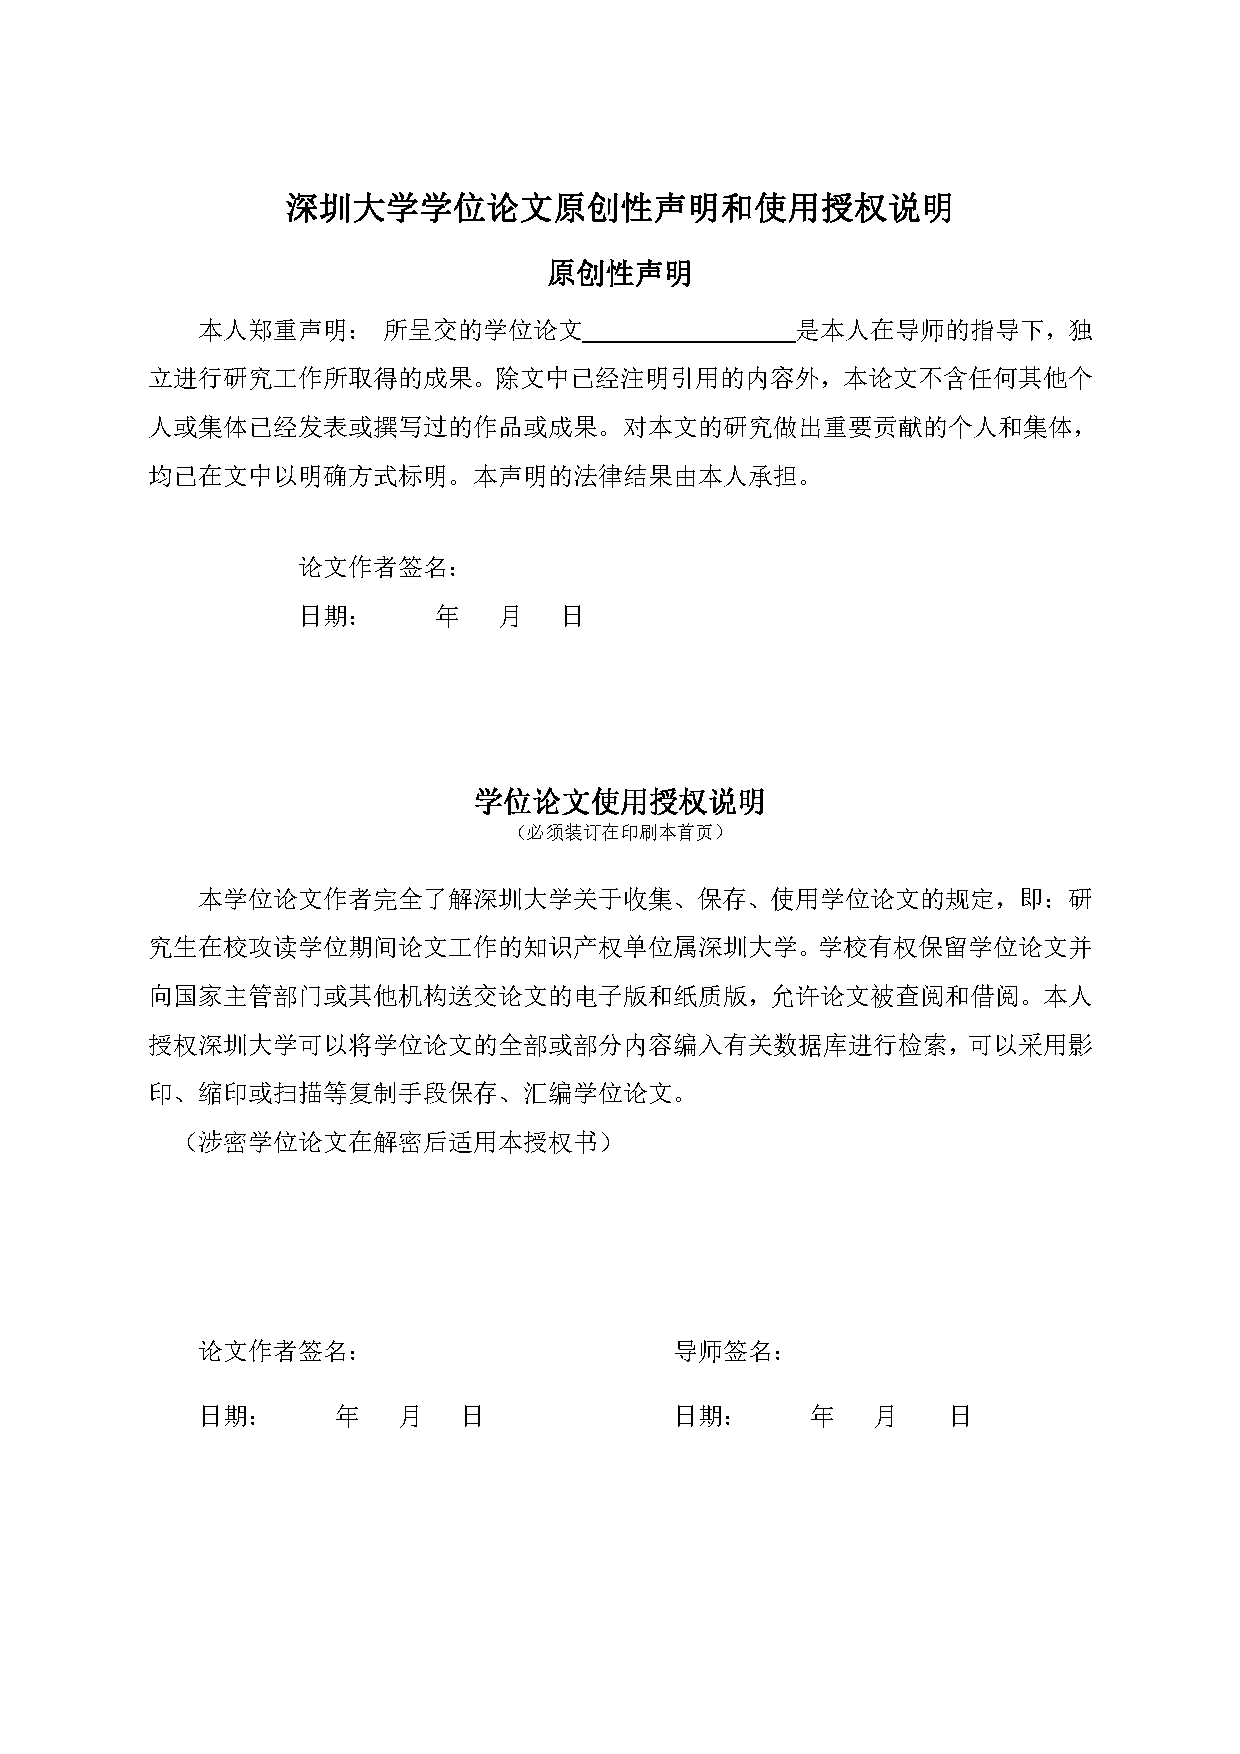
\includepdf{Copyright.pdf}
	
	
	% 如果需要打印稿,即需要打印后手写,取消该部分内容注释
	\pagestyle{fancy}
	\fancyhf{}
	\fancyfoot[C]{\song\xiaowu ~\thepage~}
	\renewcommand{\headrulewidth}{0pt}
	
	\chapter*{\song\sanhao 深圳大学学位论文原创性声明和使用授权说明}{		% modified by Jon, 原创性说明无需加入目录,使用chapter*
		\thispagestyle{empty} 		% modified by Jon: 原创性说明不需要页码
		\qquad\\
		\begin{center}\hei\xiaoer{\@declaretitle}\end{center}\par
		\song\defaultfont{\@declarecontent}\par
		\vspace*{1cm}
		{\song\xiaosi
			\@authorsigncap \makebox[2.5cm][s]{}
			\@signdatecap \makebox[2cm][s]{} 年 \makebox[1cm][s]{} 月 \makebox[1cm][s]{} 日
		}
		\vspace{0.6\baselineskip}
		\begin{center}\hei\xiaoer{\@authorizationtitle}\end{center}\par
		{
			\vspace{1.2\baselineskip}
			\song\defaultfont{\@authorizationcontent}
			\par \song\defaultfont{\@authorizationadd}
		}
		\vspace{2\baselineskip}
		
		{
			\song\xiaosi
			\@authorsigncap \makebox[3.5cm][s]{}  \@signdatecap \makebox[1.5cm][s]{} 年 \makebox[1cm][s]{} 月 \makebox[1cm][s]{} 日 \\
			\indent
			\@supervisorsigncap \makebox[3.5cm][s]{}  \@signdatecap \makebox[1.5cm][s]{} 年 \makebox[1cm][s]{} 月 \makebox[1cm][s]{} 日
		}
	}
}
\makeatother

%%%% 数据填写的部分 %%%

\declaretitle{原创性声明}
\declarecontent{
	本人郑重声明: 所呈交的学位论文\underline{《xxx》}是本人在导师的指导下,独立进行研究工作所取得的成果。除文中已经注明引用的内容外,本论文不含任何其他个人或集体已经发表或撰写过的作品或成果。对本文的研究做出重要贡献的个人和集体,均已在文中以明确方式标明。本声明的法律结果由本人承担。
}
\authorizationtitle{学位论文版权使用授权书}
\authorizationcontent{
	本学位论文作者完全了解深圳大学关于收集、保存、使用学位论文的规定,即:研究生在校攻读学位期间论文工作的知识产权单位属深圳大学。学校有权保留学位论文并向国家主管部门或其他机构送交论文的电子版和纸质版,允许论文被查阅和借阅。本人授权深圳大学可以将学位论文的全部或部分内容编入有关数据库进行检索,可以采用影印、缩印或扫描等复制手段保存、汇编学位论文。
}
\authorizationadd{(涉密学位论文在解密后适用本授权书)}
\authorsigncap{作者签名:}
\supervisorsigncap{导师签名:}
\signdatecap{签字日期:}

% 使用makecopyright生成原创性说明
\makecopyright 与 \includepdf{data/copyright.pdf} 二选一
%% !Mode:: "TeX:UTF-8"

%%%% 此处是原创性声明的格式定义,数据填写的部分在下方 %%%

\makeatletter

\def\declaretitle#1{\def\@declaretitle{#1}}\def\@declaretitle{}
\def\declarecontent#1{\def\@declarecontent{#1}}\def\@declarecontent{}
\def\authorizationtitle#1{\def\@authorizationtitle{#1}}\def\@authorizationtitle{}
\def\authorizationcontent#1{\def\@authorizationcontent{#1}}\def\@authorizationconent{}
\def\authorizationadd#1{\def\@authorizationadd{#1}}\def\@authorizationadd{}
\def\authorsigncap#1{\def\@authorsigncap{#1}}\def\@authorsigncap{}
\def\supervisorsigncap#1{\def\@supervisorsigncap{#1}}\def\@supervisorsigncap{}
\def\signdatecap#1{\def\@signdatecap{#1}}\def\@signdatecap{}

% 定义makecopyright以生成原创性说明
\def\makecopyright{
	
	\clearpage
	
	% 如果需要上传稿包含版权页,取消这部分内容注释
	%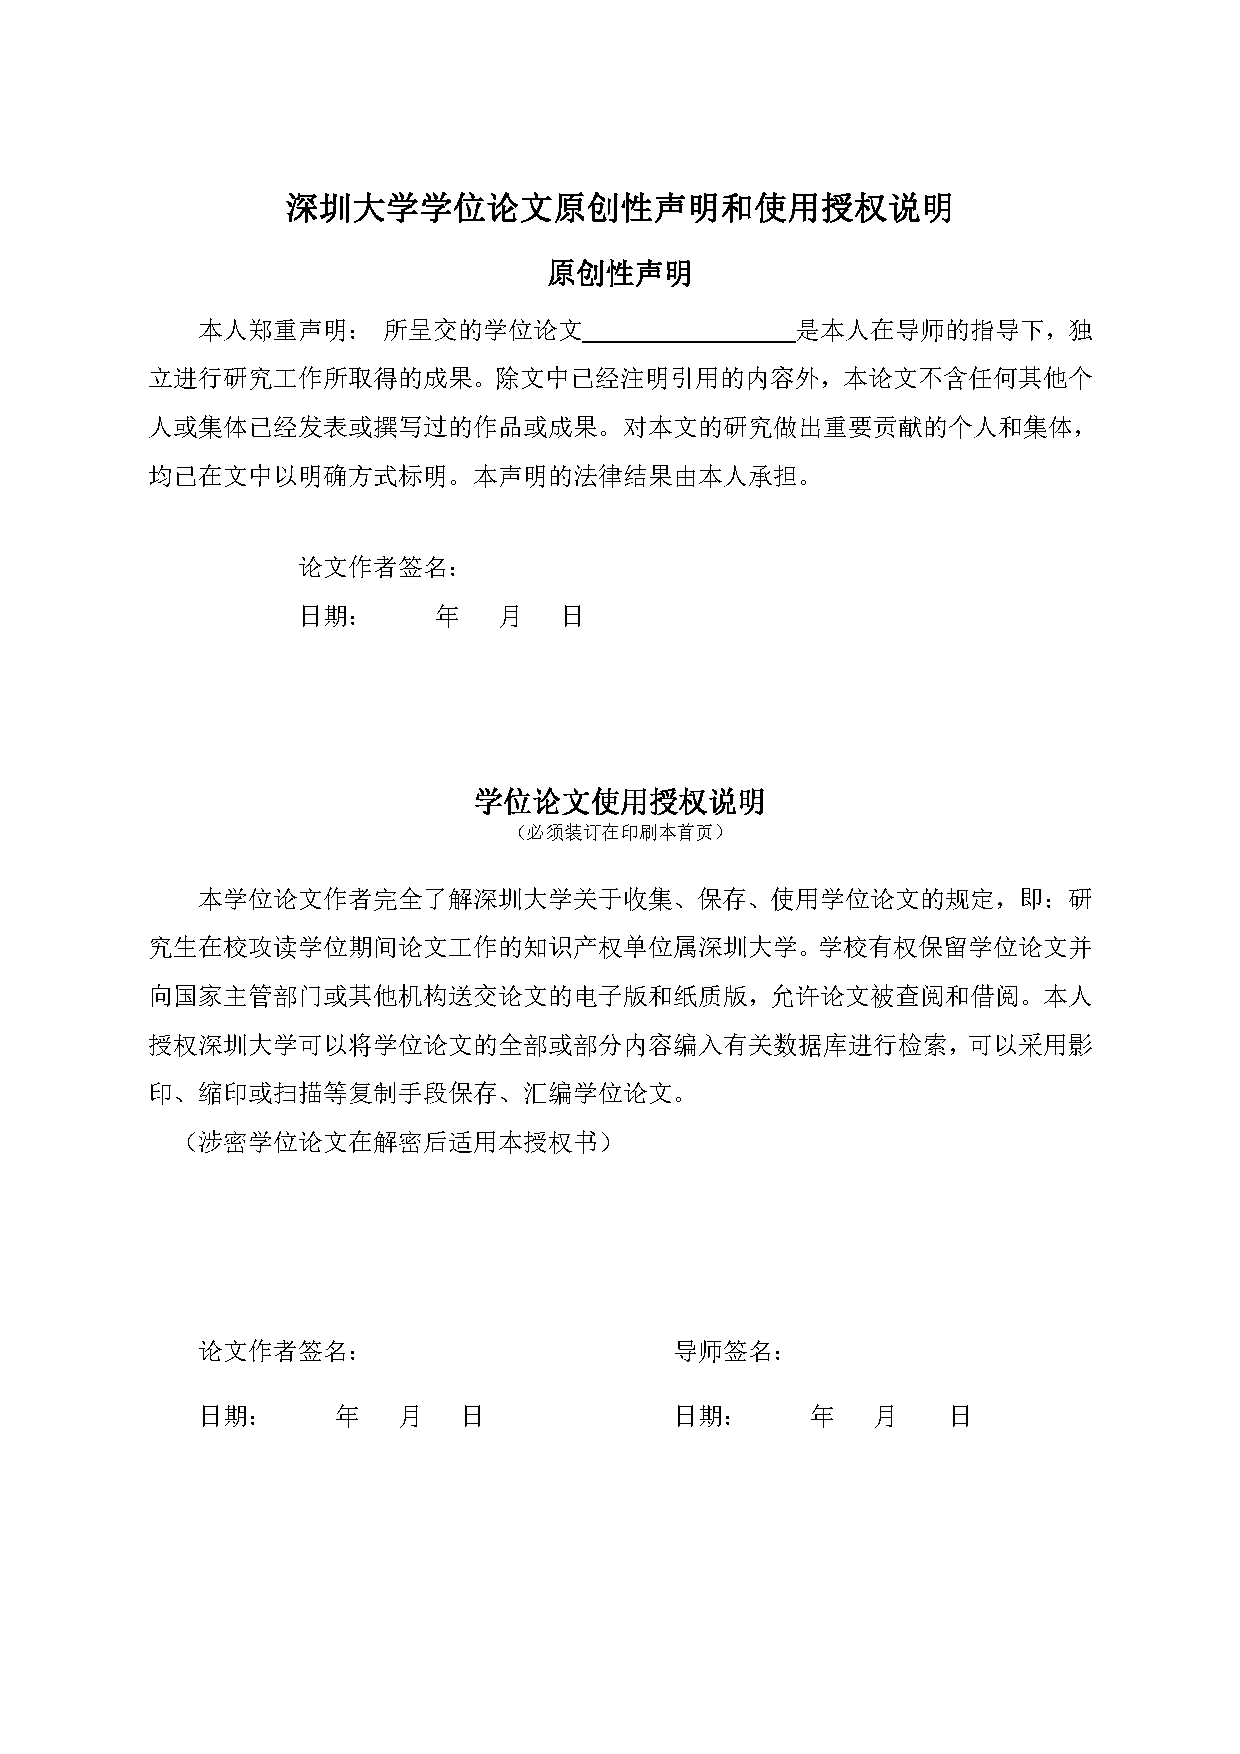
\includepdf{Copyright.pdf}
	
	
	% 如果需要打印稿,即需要打印后手写,取消该部分内容注释
	\pagestyle{fancy}
	\fancyhf{}
	\fancyfoot[C]{\song\xiaowu ~\thepage~}
	\renewcommand{\headrulewidth}{0pt}
	
	\chapter*{\song\sanhao 深圳大学学位论文原创性声明和使用授权说明}{		% modified by Jon, 原创性说明无需加入目录,使用chapter*
		\thispagestyle{empty} 		% modified by Jon: 原创性说明不需要页码
		\qquad\\
		\begin{center}\hei\xiaoer{\@declaretitle}\end{center}\par
		\song\defaultfont{\@declarecontent}\par
		\vspace*{1cm}
		{\song\xiaosi
			\@authorsigncap \makebox[2.5cm][s]{}
			\@signdatecap \makebox[2cm][s]{} 年 \makebox[1cm][s]{} 月 \makebox[1cm][s]{} 日
		}
		\vspace{0.6\baselineskip}
		\begin{center}\hei\xiaoer{\@authorizationtitle}\end{center}\par
		{
			\vspace{1.2\baselineskip}
			\song\defaultfont{\@authorizationcontent}
			\par \song\defaultfont{\@authorizationadd}
		}
		\vspace{2\baselineskip}
		
		{
			\song\xiaosi
			\@authorsigncap \makebox[3.5cm][s]{}  \@signdatecap \makebox[1.5cm][s]{} 年 \makebox[1cm][s]{} 月 \makebox[1cm][s]{} 日 \\
			\indent
			\@supervisorsigncap \makebox[3.5cm][s]{}  \@signdatecap \makebox[1.5cm][s]{} 年 \makebox[1cm][s]{} 月 \makebox[1cm][s]{} 日
		}
	}
}
\makeatother

%%%% 数据填写的部分 %%%

\declaretitle{原创性声明}
\declarecontent{
	本人郑重声明: 所呈交的学位论文\underline{《xxx》}是本人在导师的指导下,独立进行研究工作所取得的成果。除文中已经注明引用的内容外,本论文不含任何其他个人或集体已经发表或撰写过的作品或成果。对本文的研究做出重要贡献的个人和集体,均已在文中以明确方式标明。本声明的法律结果由本人承担。
}
\authorizationtitle{学位论文版权使用授权书}
\authorizationcontent{
	本学位论文作者完全了解深圳大学关于收集、保存、使用学位论文的规定,即:研究生在校攻读学位期间论文工作的知识产权单位属深圳大学。学校有权保留学位论文并向国家主管部门或其他机构送交论文的电子版和纸质版,允许论文被查阅和借阅。本人授权深圳大学可以将学位论文的全部或部分内容编入有关数据库进行检索,可以采用影印、缩印或扫描等复制手段保存、汇编学位论文。
}
\authorizationadd{(涉密学位论文在解密后适用本授权书)}
\authorsigncap{作者签名:}
\supervisorsigncap{导师签名:}
\signdatecap{签字日期:}

% 使用makecopyright生成原创性说明
\makecopyright                        % 诚信说明
\includepdf{data/copyright.pdf}             % 使用pdf文件替换原有的诚信声明data/copyright

% !Mode:: "TeX:UTF-8"

%%% 中文摘要填写部分 %%%

\cabstract{

元旦过,过元旦,元旦过完去上班;莫要吵,莫要闹,祝福短信送不完。元旦过完是新年,问候依旧在心间,借着元旦的余热提前祝你新年快乐!

团团圆圆,圆你美梦,快快乐乐,乐享人生,健健康康,平安如意,幸幸福福,逍遥自在,热热闹闹,欢天喜地,元旦快乐,愿您开心!

一年有365个日出,我心有365个祝福,一年有365个日落,我心有365个心愿,祝你健健康康另一个365,愿你平平安安另一个365,元旦节快乐!

快乐时我给你祝福,失意时给你安抚,友情是最大的财富,幸福蕴含在知足。新的一年,让我们共同祝福,元旦快乐!快乐永远!新的一年梦想实现!

元旦的曙光就要来了,请对着蓝天微笑一下。我要剪裁2011个开心时光,为你缝成2012件幸福衣裳。别忘了,即使活得很现实,也要想得很美好。

喜悦,在心中荡漾;笑容,在脸颊洋溢;歌声,在悠扬回荡;舞步,在惬意游走;礼花,在尽情绽放;祝福,在频频发送。朋友,元旦快乐!祝你幸福,阖家欢乐!

元旦将来到,我心费思量。朋友关系好,送个什么好。我无多钱财,也没中彩票。短信送祝福,礼轻情意重。祝你轻轻松松无烦恼,快快乐乐过元旦!

元旦过,过元旦,元旦过完去上班;莫要吵,莫要闹,祝福短信送不完。元旦过完是新年,问候依旧在心间,借着元旦的余热提前祝你新年快乐!

团团圆圆,圆你美梦,快快乐乐,乐享人生,健健康康,平安如意,幸幸福福,逍遥自在,热热闹闹,欢天喜地,元旦快乐,愿您开心!

一年有365个日出,我心有365个祝福,一年有365个日落,我心有365个心愿,祝你健健康康另一个365,愿你平平安安另一个365,元旦节快乐!

快乐时我给你祝福,失意时给你安抚,友情是最大的财富,幸福蕴含在知足。新的一年,让我们共同祝福,元旦快乐!快乐永远!新的一年梦想实现!

元旦的曙光就要来了,请对着蓝天微笑一下。我要剪裁2011个开心时光,为你缝成2012件幸福衣裳。别忘了,即使活得很现实,也要想得很美好。

喜悦,在心中荡漾;笑容,在脸颊洋溢;歌声,在悠扬回荡;舞步,在惬意游走;礼花,在尽情绽放;祝福,在频频发送。朋友,元旦快乐!祝你幸福,阖家欢乐!

元旦将来到,我心费思量。朋友关系好,送个什么好。我无多钱财,也没中彩票。短信送祝福,礼轻情意重。祝你轻轻松松无烦恼,快快乐乐过元旦!

元旦过,过元旦,元旦过完去上班;莫要吵,莫要闹,祝福短信送不完。元旦过完是新年,问候依旧在心间,借着元旦的余热提前祝你新年快乐!

团团圆圆,圆你美梦,快快乐乐,乐享人生,健健康康,平安如意,幸幸福福,逍遥自在,热热闹闹,欢天喜地,元旦快乐,愿您开心!

一年有365个日出,我心有365个祝福,一年有365个日落,我心有365个心愿,祝你健健康康另一个365,愿你平平安安另一个365,元旦节快乐!

快乐时我给你祝福,失意时给你安抚,友情是最大的财富,幸福蕴含在知足。新的一年,让我们共同祝福,元旦快乐!快乐永远!新的一年梦想实现!

元旦的曙光就要来了,请对着蓝天微笑一下。我要剪裁2011个开心时光,为你缝成2012件幸福衣裳。别忘了,即使活得很现实,也要想得很美好。

喜悦,在心中荡漾;笑容,在脸颊洋溢;歌声,在悠扬回荡;舞步,在惬意游走;礼花,在尽情绽放;祝福,在频频发送。朋友,元旦快乐!祝你幸福,阖家欢乐!

元旦将来到,我心费思量。朋友关系好,送个什么好。我无多钱财,也没中彩票。短信送祝福,礼轻情意重。祝你轻轻松松无烦恼,快快乐乐过元旦!


}
\ckeywords{关键字1;~~关键字2;~~关键字3}

% 使用makecnabstract生成中文摘要
\makecnabstract						% 中文摘要
% !Mode:: "TeX:UTF-8"

%%% 此处是英文摘要的格式设置,数据部分在下面 %%%
\makeatletter

\long\def\enabstract#1{\long\def\@enabstract{#1}}\long\def\@enabstract{}
\def\enkeywords#1{\def\@enkeywords{#1}}\def\@enkeywords{}
\def\enpageheader#1{\def\@enpageheader{#1}}\def\@enpageheader{}

% 定义makeenabstract以生成英文摘要
\def\makeenabstract{
	
	\clearpage
	
	% 使用fancy来设置页眉页脚,自定义了新的格式——englishAbstract
	\pagestyle{fancy}
	\fancypagestyle{englishAbstract}{
		\fancyhead[C]{\wuhao \@enpageheader}		% 使用英文论文名称作为页眉
		\fancyfoot[C]{\song\wuhao ~\thepage~}
	}
	
	\addcontentsline{toc}{chapter}{Abstract}
	\chapter*{\centering\erhao \bf{Abstract}}		% 二号
	%\vspace{\baselineskip}
	\@enabstract
	\thispagestyle{englishAbstract}		% modified by Jon: 应用englishAbstract
	\vspace{\baselineskip}
	
	%\hangafter=1\hangindent=60pt\noindent  %如果取消该行注释,KEY WORDS换行时将会自动缩进
	\noindent
	{\xiaosi\textbf{Key Words:} \@enkeywords}
	
}
\makeatother


%%% 英文摘要数据部分 %%%

\enabstract{英文摘要写在此处}
\enpageheader{英文页眉标题}
\enkeywords{keyworkds1;~~keyworkds2;~~keyworkds3}

% 使用makeenabstract生成英文摘要
\makeenabstract						% 英文摘要

\clearpage
\pagestyle{empty}		% modified by Jon: 去掉页眉页脚
% 目录
\renewcommand{\contentsname}{\erhao\song\bfseries\hspace*{\fill}目\quad 录\hspace*{\fill}}    % 设置“目录”二字的格式
\tableofcontents                           % 中文目录

\clearpage
\cleardoublepage

% 正文部分
\defaultfont
\pagestyle{plain}
\mainmatter\sloppy\raggedbottom
%\renewcommand{\ALC@linenosize}{\xiaosi}
\renewcommand\arraystretch{1.5}
\setlength{\intextsep}{2pt}
\setlength{\abovecaptionskip}{2pt}
\setlength{\belowcaptionskip}{2pt}

% 内容比较多的时候,编译速度较慢,可以将不同章节放在不同文件中,注释掉其他章节,只编译正在撰写的章节,以提升编译速度
% !Mode:: "TeX:UTF-8"

\chapter{绪论}

\section{引言}

测试引言,可以自动首行缩进。测试引言,可以自动首行缩进。测试引言,可以自动首行缩进。测试引言,可以自动首行缩进。测试引言,可以自动首行缩进。这是引用测试\cite{barnes2009patchmatch}\cite{barnes2009patchmatch2}\cite{barnes2009patchmatch3}\cite{barnes2009patchmatch4}\cite{barnes2009patchmatch5}\cite{barnes2009patchmatch6}\cite{barnes2009patchmatch7}\cite{barnes2009patchmatch8}\cite{barnes2009patchmatch9}\cite{barnes2009patchmatch10}\cite{barnes2009patchmatch11}\cite{barnes2009patchmatch12}\cite{barnes2009patchmatch13}\cite{barnes2009patchmatch14}\cite{barnes2009patchmatch15}\cite{barnes2009patchmatch16}\cite{barnes2009patchmatch17}\cite{barnes2009patchmatch18}。

元旦过,过元旦,元旦过完去上班;莫要吵,莫要闹,祝福短信送不完。元旦过完是新年,问候依旧在心间,借着元旦的余热提前祝你新年快乐!

团团圆圆,圆你美梦,快快乐乐,乐享人生,健健康康,平安如意,幸幸福福,逍遥自在,热热闹闹,欢天喜地,元旦快乐,愿您开心!

一年有365个日出,我心有365个祝福,一年有365个日落,我心有365个心愿,祝你健健康康另一个365,愿你平平安安另一个365,元旦节快乐!

快乐时我给你祝福,失意时给你安抚,友情是最大的财富,幸福蕴含在知足。新的一年,让我们共同祝福,元旦快乐!快乐永远!新的一年梦想实现!

元旦的曙光就要来了,请对着蓝天微笑一下。我要剪裁2011个开心时光,为你缝成2012件幸福衣裳。别忘了,即使活得很现实,也要想得很美好。

喜悦,在心中荡漾;笑容,在脸颊洋溢;歌声,在悠扬回荡;舞步,在惬意游走;礼花,在尽情绽放;祝福,在频频发送。朋友,元旦快乐!祝你幸福,阖家欢乐!

元旦将来到,我心费思量。朋友关系好,送个什么好。我无多钱财,也没中彩票。短信送祝福,礼轻情意重。祝你轻轻松松无烦恼,快快乐乐过元旦!

\section{研究现状}

元旦过,过元旦,元旦过完去上班;莫要吵,莫要闹,祝福短信送不完。元旦过完是新年,问候依旧在心间,借着元旦的余热提前祝你新年快乐!

团团圆圆,圆你美梦,快快乐乐,乐享人生,健健康康,平安如意,幸幸福福,逍遥自在,热热闹闹,欢天喜地,元旦快乐,愿您开心!

一年有365个日出,我心有365个祝福,一年有365个日落,我心有365个心愿,祝你健健康康另一个365,愿你平平安安另一个365,元旦节快乐!

快乐时我给你祝福,失意时给你安抚,友情是最大的财富,幸福蕴含在知足。新的一年,让我们共同祝福,元旦快乐!快乐永远!新的一年梦想实现!

元旦的曙光就要来了,请对着蓝天微笑一下。我要剪裁2011个开心时光,为你缝成2012件幸福衣裳。别忘了,即使活得很现实,也要想得很美好。

喜悦,在心中荡漾;笑容,在脸颊洋溢;歌声,在悠扬回荡;舞步,在惬意游走;礼花,在尽情绽放;祝福,在频频发送。朋友,元旦快乐!祝你幸福,阖家欢乐!

元旦将来到,我心费思量。朋友关系好,送个什么好。我无多钱财,也没中彩票。短信送祝福,礼轻情意重。祝你轻轻松松无烦恼,快快乐乐过元旦!

\subsection{小节x}

元旦过,过元旦,元旦过完去上班;莫要吵,莫要闹,祝福短信送不完。元旦过完是新年,问候依旧在心间,借着元旦的余热提前祝你新年快乐!

\subsection{小节x}

元旦过,过元旦,元旦过完去上班;莫要吵,莫要闹,祝福短信送不完。元旦过完是新年,问候依旧在心间,借着元旦的余热提前祝你新年快乐!

\subsection{小节x}

元旦过,过元旦,元旦过完去上班;莫要吵,莫要闹,祝福短信送不完。元旦过完是新年,问候依旧在心间,借着元旦的余热提前祝你新年快乐!

\subsection{小节x}

元旦过,过元旦,元旦过完去上班;莫要吵,莫要闹,祝福短信送不完。元旦过完是新年,问候依旧在心间,借着元旦的余热提前祝你新年快乐!

\subsection{小节x}

元旦过,过元旦,元旦过完去上班;莫要吵,莫要闹,祝福短信送不完。元旦过完是新年,问候依旧在心间,借着元旦的余热提前祝你新年快乐!

\subsection{小节x}

元旦过,过元旦,元旦过完去上班;莫要吵,莫要闹,祝福短信送不完。元旦过完是新年,问候依旧在心间,借着元旦的余热提前祝你新年快乐!

\subsection{小节x}

元旦过,过元旦,元旦过完去上班;莫要吵,莫要闹,祝福短信送不完。元旦过完是新年,问候依旧在心间,借着元旦的余热提前祝你新年快乐!

\subsection{小节x}

元旦过,过元旦,元旦过完去上班;莫要吵,莫要闹,祝福短信送不完。元旦过完是新年,问候依旧在心间,借着元旦的余热提前祝你新年快乐!

\subsection{小节x}

元旦过,过元旦,元旦过完去上班;莫要吵,莫要闹,祝福短信送不完。元旦过完是新年,问候依旧在心间,借着元旦的余热提前祝你新年快乐!

\subsection{小节x}

元旦过,过元旦,元旦过完去上班;莫要吵,莫要闹,祝福短信送不完。元旦过完是新年,问候依旧在心间,借着元旦的余热提前祝你新年快乐!

\subsection{小节x}

元旦过,过元旦,元旦过完去上班;莫要吵,莫要闹,祝福短信送不完。元旦过完是新年,问候依旧在心间,借着元旦的余热提前祝你新年快乐!

\subsection{小节x}

元旦过,过元旦,元旦过完去上班;莫要吵,莫要闹,祝福短信送不完。元旦过完是新年,问候依旧在心间,借着元旦的余热提前祝你新年快乐!

\subsection{小节x}

元旦过,过元旦,元旦过完去上班;莫要吵,莫要闹,祝福短信送不完。元旦过完是新年,问候依旧在心间,借着元旦的余热提前祝你新年快乐!

\subsection{小节x}

元旦过,过元旦,元旦过完去上班;莫要吵,莫要闹,祝福短信送不完。元旦过完是新年,问候依旧在心间,借着元旦的余热提前祝你新年快乐!

\subsection{小节x}

元旦过,过元旦,元旦过完去上班;莫要吵,莫要闹,祝福短信送不完。元旦过完是新年,问候依旧在心间,借着元旦的余热提前祝你新年快乐!

\subsection{小节x}

元旦过,过元旦,元旦过完去上班;莫要吵,莫要闹,祝福短信送不完。元旦过完是新年,问候依旧在心间,借着元旦的余热提前祝你新年快乐!

\subsection{小节x}

元旦过,过元旦,元旦过完去上班;莫要吵,莫要闹,祝福短信送不完。元旦过完是新年,问候依旧在心间,借着元旦的余热提前祝你新年快乐!

\subsection{小节x}

元旦过,过元旦,元旦过完去上班;莫要吵,莫要闹,祝福短信送不完。元旦过完是新年,问候依旧在心间,借着元旦的余热提前祝你新年快乐!

\subsection{小节x}

元旦过,过元旦,元旦过完去上班;莫要吵,莫要闹,祝福短信送不完。元旦过完是新年,问候依旧在心间,借着元旦的余热提前祝你新年快乐!

\subsection{小节x}

元旦过,过元旦,元旦过完去上班;莫要吵,莫要闹,祝福短信送不完。元旦过完是新年,问候依旧在心间,借着元旦的余热提前祝你新年快乐!

\subsection{小节x}

元旦过,过元旦,元旦过完去上班;莫要吵,莫要闹,祝福短信送不完。元旦过完是新年,问候依旧在心间,借着元旦的余热提前祝你新年快乐!

\subsection{小节x}

元旦过,过元旦,元旦过完去上班;莫要吵,莫要闹,祝福短信送不完。元旦过完是新年,问候依旧在心间,借着元旦的余热提前祝你新年快乐!

\subsection{小节x}

元旦过,过元旦,元旦过完去上班;莫要吵,莫要闹,祝福短信送不完。元旦过完是新年,问候依旧在心间,借着元旦的余热提前祝你新年快乐!

\subsection{小节x}

元旦过,过元旦,元旦过完去上班;莫要吵,莫要闹,祝福短信送不完。元旦过完是新年,问候依旧在心间,借着元旦的余热提前祝你新年快乐!

\subsection{小节x}

元旦过,过元旦,元旦过完去上班;莫要吵,莫要闹,祝福短信送不完。元旦过完是新年,问候依旧在心间,借着元旦的余热提前祝你新年快乐!

\subsection{小节x}

元旦过,过元旦,元旦过完去上班;莫要吵,莫要闹,祝福短信送不完。元旦过完是新年,问候依旧在心间,借着元旦的余热提前祝你新年快乐!

\subsection{小节x}

元旦过,过元旦,元旦过完去上班;莫要吵,莫要闹,祝福短信送不完。元旦过完是新年,问候依旧在心间,借着元旦的余热提前祝你新年快乐!

\subsection{小节x}

元旦过,过元旦,元旦过完去上班;莫要吵,莫要闹,祝福短信送不完。元旦过完是新年,问候依旧在心间,借着元旦的余热提前祝你新年快乐!

\subsection{小节x}

元旦过,过元旦,元旦过完去上班;莫要吵,莫要闹,祝福短信送不完。元旦过完是新年,问候依旧在心间,借着元旦的余热提前祝你新年快乐!

\subsection{小节x}

元旦过,过元旦,元旦过完去上班;莫要吵,莫要闹,祝福短信送不完。元旦过完是新年,问候依旧在心间,借着元旦的余热提前祝你新年快乐!

\subsection{小节x}

元旦过,过元旦,元旦过完去上班;莫要吵,莫要闹,祝福短信送不完。元旦过完是新年,问候依旧在心间,借着元旦的余热提前祝你新年快乐!

\subsection{小节x}

元旦过,过元旦,元旦过完去上班;莫要吵,莫要闹,祝福短信送不完。元旦过完是新年,问候依旧在心间,借着元旦的余热提前祝你新年快乐!

\subsection{小节x}

元旦过,过元旦,元旦过完去上班;莫要吵,莫要闹,祝福短信送不完。元旦过完是新年,问候依旧在心间,借着元旦的余热提前祝你新年快乐!

\subsection{小节x}

元旦过,过元旦,元旦过完去上班;莫要吵,莫要闹,祝福短信送不完。元旦过完是新年,问候依旧在心间,借着元旦的余热提前祝你新年快乐!

\subsection{小节x}

元旦过,过元旦,元旦过完去上班;莫要吵,莫要闹,祝福短信送不完。元旦过完是新年,问候依旧在心间,借着元旦的余热提前祝你新年快乐!

\subsection{小节x}

元旦过,过元旦,元旦过完去上班;莫要吵,莫要闹,祝福短信送不完。元旦过完是新年,问候依旧在心间,借着元旦的余热提前祝你新年快乐!

\subsection{小节x}

元旦过,过元旦,元旦过完去上班;莫要吵,莫要闹,祝福短信送不完。元旦过完是新年,问候依旧在心间,借着元旦的余热提前祝你新年快乐!

\subsection{小节x}

元旦过,过元旦,元旦过完去上班;莫要吵,莫要闹,祝福短信送不完。元旦过完是新年,问候依旧在心间,借着元旦的余热提前祝你新年快乐!

\subsection{小节x}

元旦过,过元旦,元旦过完去上班;莫要吵,莫要闹,祝福短信送不完。元旦过完是新年,问候依旧在心间,借着元旦的余热提前祝你新年快乐!

\subsection{小节x}

元旦过,过元旦,元旦过完去上班;莫要吵,莫要闹,祝福短信送不完。元旦过完是新年,问候依旧在心间,借着元旦的余热提前祝你新年快乐!

\subsection{小节x}

元旦过,过元旦,元旦过完去上班;莫要吵,莫要闹,祝福短信送不完。元旦过完是新年,问候依旧在心间,借着元旦的余热提前祝你新年快乐!

\subsection{小节x}

元旦过,过元旦,元旦过完去上班;莫要吵,莫要闹,祝福短信送不完。元旦过完是新年,问候依旧在心间,借着元旦的余热提前祝你新年快乐!

\subsection{小节x}

元旦过,过元旦,元旦过完去上班;莫要吵,莫要闹,祝福短信送不完。元旦过完是新年,问候依旧在心间,借着元旦的余热提前祝你新年快乐!

\subsection{小节x}

元旦过,过元旦,元旦过完去上班;莫要吵,莫要闹,祝福短信送不完。元旦过完是新年,问候依旧在心间,借着元旦的余热提前祝你新年快乐!


\section{本文主要方法及思路}

元旦过,过元旦,元旦过完去上班;莫要吵,莫要闹,祝福短信送不完。元旦过完是新年,问候依旧在心间,借着元旦的余热提前祝你新年快乐!

团团圆圆,圆你美梦,快快乐乐,乐享人生,健健康康,平安如意,幸幸福福,逍遥自在,热热闹闹,欢天喜地,元旦快乐,愿您开心!

一年有365个日出,我心有365个祝福,一年有365个日落,我心有365个心愿,祝你健健康康另一个365,愿你平平安安另一个365,元旦节快乐!

快乐时我给你祝福,失意时给你安抚,友情是最大的财富,幸福蕴含在知足。新的一年,让我们共同祝福,元旦快乐!快乐永远!新的一年梦想实现!

元旦的曙光就要来了,请对着蓝天微笑一下。我要剪裁2011个开心时光,为你缝成2012件幸福衣裳。别忘了,即使活得很现实,也要想得很美好。

喜悦,在心中荡漾;笑容,在脸颊洋溢;歌声,在悠扬回荡;舞步,在惬意游走;礼花,在尽情绽放;祝福,在频频发送。朋友,元旦快乐!祝你幸福,阖家欢乐!

元旦将来到,我心费思量。朋友关系好,送个什么好。我无多钱财,也没中彩票。短信送祝福,礼轻情意重。祝你轻轻松松无烦恼,快快乐乐过元旦!

\section{论文结构}

元旦过,过元旦,元旦过完去上班;莫要吵,莫要闹,祝福短信送不完。元旦过完是新年,问候依旧在心间,借着元旦的余热提前祝你新年快乐!

团团圆圆,圆你美梦,快快乐乐,乐享人生,健健康康,平安如意,幸幸福福,逍遥自在,热热闹闹,欢天喜地,元旦快乐,愿您开心!

一年有365个日出,我心有365个祝福,一年有365个日落,我心有365个心愿,祝你健健康康另一个365,愿你平平安安另一个365,元旦节快乐!

快乐时我给你祝福,失意时给你安抚,友情是最大的财富,幸福蕴含在知足。新的一年,让我们共同祝福,元旦快乐!快乐永远!新的一年梦想实现!

元旦的曙光就要来了,请对着蓝天微笑一下。我要剪裁2011个开心时光,为你缝成2012件幸福衣裳。别忘了,即使活得很现实,也要想得很美好。

喜悦,在心中荡漾;笑容,在脸颊洋溢;歌声,在悠扬回荡;舞步,在惬意游走;礼花,在尽情绽放;祝福,在频频发送。朋友,元旦快乐!祝你幸福,阖家欢乐!

元旦将来到,我心费思量。朋友关系好,送个什么好。我无多钱财,也没中彩票。短信送祝福,礼轻情意重。祝你轻轻松松无烦恼,快快乐乐过元旦!




 							
% !Mode:: "TeX:UTF-8"
\chapter{章节名称}
本章主要介绍
\section{小节名称}

\section{本章小结}


% !Mode:: "TeX:UTF-8"
\chapter{章节名称}
本章主要介绍
\section{小节名称}

\section{本章小结}

						
% !Mode:: "TeX:UTF-8"

\addcontentsline{toc}{chapter}{结\quad 论} %添加到目录中
\chapter*{结\quad 论}
xxx,本文主要工作




% 参考文献
% 若是要对参考文献进行重新编译,需要先使用clean.bat或是clean.sh清除辅助文件
\defaultfont
\bibliographystyle{HNUThesis}
\phantomsection
\addcontentsline{toc}{chapter}{参考文献}          	% 参考文献加入到中文目录
%\nocite{*}                                        	% 若将此命令屏蔽掉,则未引用的文献不会出现在文后的参考文献中。 
\bibliography{references}					

\renewcommand\thefigure{A.\arabic{figure}}			% 将附录中的图像的id的章节num设置为A
% !Mode:: "TeX:UTF-8"

\newenvironment{theappendix}{\wuhao\song}

\addcontentsline{toc}{chapter}{附录}%添加到目录中
\chapter*{\centering\xiaosan\hei\bfseries 附\quad 录}

\begin{theappendix}


\end{theappendix}

                   			% 附录
% !Mode:: "TeX:UTF-8"

\newenvironment{theacknowledgements}{\wuhao\song}

\addcontentsline{toc}{chapter}{致谢}%添加到目录中
\chapter*{\centering\xiaosan\hei\bfseries 致\quad 谢}

\begin{theacknowledgements}
	
元旦过,过元旦,元旦过完去上班;莫要吵,莫要闹,祝福短信送不完。元旦过完是新年,问候依旧在心间,借着元旦的余热提前祝你新年快乐!

团团圆圆,圆你美梦,快快乐乐,乐享人生,健健康康,平安如意,幸幸福福,逍遥自在,热热闹闹,欢天喜地,元旦快乐,愿您开心!

一年有365个日出,我心有365个祝福,一年有365个日落,我心有365个心愿,祝你健健康康另一个365,愿你平平安安另一个365,元旦节快乐!

快乐时我给你祝福,失意时给你安抚,友情是最大的财富,幸福蕴含在知足。新的一年,让我们共同祝福,元旦快乐!快乐永远!新的一年梦想实现!

元旦的曙光就要来了,请对着蓝天微笑一下。我要剪裁2011个开心时光,为你缝成2012件幸福衣裳。别忘了,即使活得很现实,也要想得很美好。

喜悦,在心中荡漾;笑容,在脸颊洋溢;歌声,在悠扬回荡;舞步,在惬意游走;礼花,在尽情绽放;祝福,在频频发送。朋友,元旦快乐!祝你幸福,阖家欢乐!

元旦将来到,我心费思量。朋友关系好,送个什么好。我无多钱财,也没中彩票。短信送祝福,礼轻情意重。祝你轻轻松松无烦恼,快快乐乐过元旦!

元旦过,过元旦,元旦过完去上班;莫要吵,莫要闹,祝福短信送不完。元旦过完是新年,问候依旧在心间,借着元旦的余热提前祝你新年快乐!

团团圆圆,圆你美梦,快快乐乐,乐享人生,健健康康,平安如意,幸幸福福,逍遥自在,热热闹闹,欢天喜地,元旦快乐,愿您开心!

一年有365个日出,我心有365个祝福,一年有365个日落,我心有365个心愿,祝你健健康康另一个365,愿你平平安安另一个365,元旦节快乐!

快乐时我给你祝福,失意时给你安抚,友情是最大的财富,幸福蕴含在知足。新的一年,让我们共同祝福,元旦快乐!快乐永远!新的一年梦想实现!

元旦的曙光就要来了,请对着蓝天微笑一下。我要剪裁2011个开心时光,为你缝成2012件幸福衣裳。别忘了,即使活得很现实,也要想得很美好。

喜悦,在心中荡漾;笑容,在脸颊洋溢;歌声,在悠扬回荡;舞步,在惬意游走;礼花,在尽情绽放;祝福,在频频发送。朋友,元旦快乐!祝你幸福,阖家欢乐!

元旦将来到,我心费思量。朋友关系好,送个什么好。我无多钱财,也没中彩票。短信送祝福,礼轻情意重。祝你轻轻松松无烦恼,快快乐乐过元旦!

元旦过,过元旦,元旦过完去上班;莫要吵,莫要闹,祝福短信送不完。元旦过完是新年,问候依旧在心间,借着元旦的余热提前祝你新年快乐!

团团圆圆,圆你美梦,快快乐乐,乐享人生,健健康康,平安如意,幸幸福福,逍遥自在,热热闹闹,欢天喜地,元旦快乐,愿您开心!

一年有365个日出,我心有365个祝福,一年有365个日落,我心有365个心愿,祝你健健康康另一个365,愿你平平安安另一个365,元旦节快乐!

快乐时我给你祝福,失意时给你安抚,友情是最大的财富,幸福蕴含在知足。新的一年,让我们共同祝福,元旦快乐!快乐永远!新的一年梦想实现!

元旦的曙光就要来了,请对着蓝天微笑一下。我要剪裁2011个开心时光,为你缝成2012件幸福衣裳。别忘了,即使活得很现实,也要想得很美好。

喜悦,在心中荡漾;笑容,在脸颊洋溢;歌声,在悠扬回荡;舞步,在惬意游走;礼花,在尽情绽放;祝福,在频频发送。朋友,元旦快乐!祝你幸福,阖家欢乐!

元旦将来到,我心费思量。朋友关系好,送个什么好。我无多钱财,也没中彩票。短信送祝福,礼轻情意重。祝你轻轻松松无烦恼,快快乐乐过元旦!

\rightline{姓名}

\rightline{二零二零年三月 于地名}

\end{theacknowledgements}





						% 致谢
% !Mode:: "TeX:UTF-8"

\newenvironment{thepublications}{\wuhao\song}

\addcontentsline{toc}{chapter}{攻读硕士学位期间的研究成果}%添加到目录中
\chapter*{\centering\xiaosan\hei\bfseries 攻读硕士士学位期间的研究成果}

\begin{thepublications}

\setlength{\parindent}{0em}
\begin{publist}
	\item	发的论文或者专利
\end{publist}

\vfill
\hangafter=1\hangindent=2em\noindent

\setlength{\parindent}{2em}

\end{thepublications}

							% 研究成果
\clearpage

\end{CJK*}                                        	% 结束中文字体使用
\end{document}                                    	% 结束全文
